\chapter{Конструкторский раздел}
\label{cha:design}
В данном разделе будет рассмотрена схема реализованного алгоритма шифрования и описан способом его конвейеризации.

\section{Схемы алгоритмов}
В программе реализовано шифрование строк используя шифр цезаря и XOR-шифр, на рисунках \ref{fig:caesar} и \ref{fig:xor} представлены схемы выбранных алгоритмов шифрования.
\begin{figure}[H]
	\centering
	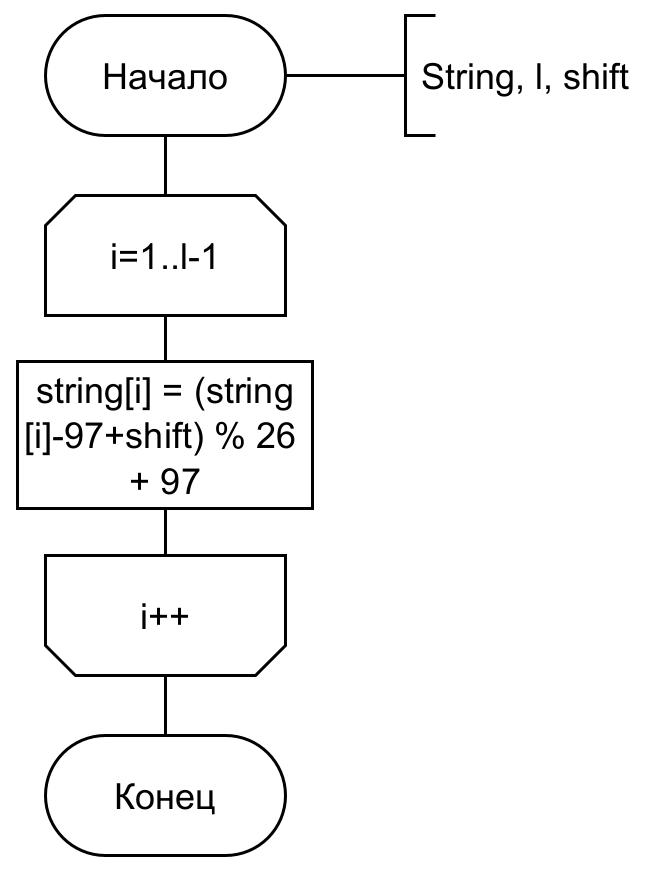
\includegraphics[width=0.5\linewidth]{src/caesar}
	\caption{Алгоритм шифрования Цезаря}
	\label{fig:caesar}
\end{figure}
\begin{figure}[H]
	\centering
	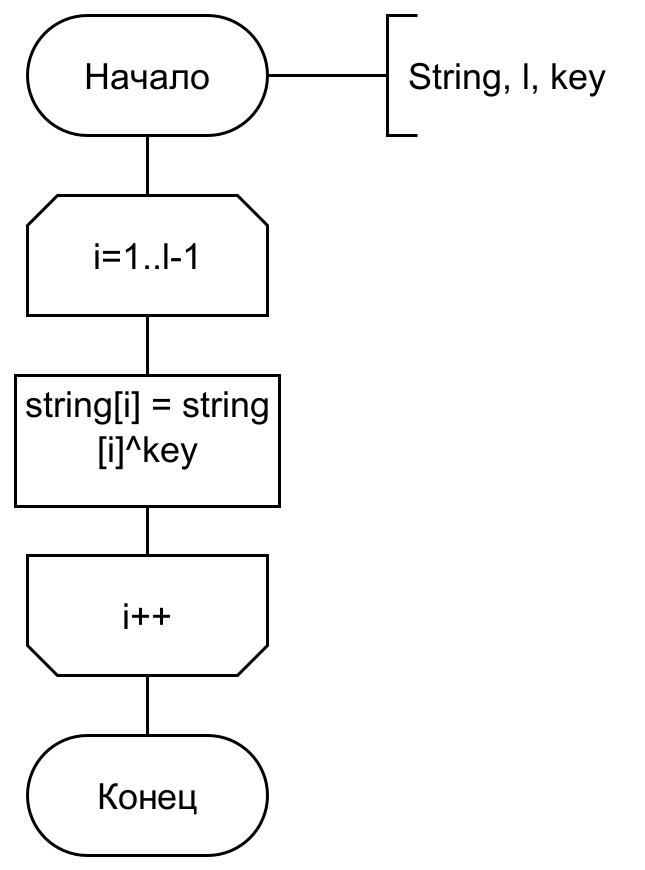
\includegraphics[width=0.5\linewidth]{src/xor}
	\caption{Алгоритм XOR-шифрования}
	\label{fig:xor}
\end{figure}

\section{Конвейеризация задачи}
Алгоритм шифрования с программе разбит на 3 этапа: сначала к строке применяется шифр Цезаря, затем XOR-шифр и снова шифр Цезаря. Каждый из этих этапов выделен в отличную стадию выполнения конвейера. Таким образом главный поток при запуске вызывает генератор заявок, после чего создаёт 3 потока, каждому из которых выделяет определённую задачу.

\section{Вывод}
В данном разделе была рассмотрены схемы алгоритмов шифра Цезаря и XOR-шифра, описана схема конвейеризации поставленной задачи.